\documentclass{article}

%\usepackage[german]{babel}
\usepackage[pdftex]{color,graphicx}
\usepackage{verbatim}

\usepackage{page}

\begin{document}

\title{Converting Gambit Grids for Semtex}
\author{%
Erik Torres, J\"org Stiller \\[5mm] 
TU Dresden, Institute for Aerospace Engineering (ILR) \\ 
01062 Dresden, Germany}
\date{\today}
\maketitle

\section{Introduction}

This guide gives a brief overview on the conversion of gambit grid
files to semtex session files using gambit2semtex. 
The following features are supported:
\begin{itemize}
 \item Import of unstructured quadrilateral grids.
 \item Support of periodic boundaries.
 \item Support of semtex curves of the types \verb|ARC| and \verb|SPLINE|.
 \item Reuse or automated generation of spline data.
\end{itemize}
A drawback of the current version is the large overhead in the sources, which results from the fact that the code was adopted from another application.

\section{Installation}

To build the conversion program you need a Fortran\,95 compliant compiler. 
Possible choices are the freely available \emph{g95} or \emph{gfortran}, 
however any other up-to-date compiler (e.g. Intel's \emph{ifort}) should work 
as well. 
Change to the source directory \verb|src| and edit \texttt{GNUmakefile} 
such that the variables \verb|FC| (referencing the compiler) and \verb|FOPTS|
(compiler options) are initialised properly. To build the program just type 

\begin{verbatim}
> make
\end{verbatim}

For generating the session file proceed as follows: 
\begin{enumerate} 
 \item Produce a suitable meshfile using gambit.
 \item Create the input file for gambit2semtex and execute the program.
 \item Add the problem specific sections to the resulting session file. 
\end{enumerate}

Some import details are discussed in the following sections. The corresponding 
example files are located in the directory \verb|example|.


\section{Preparing the grid file}

It is beyond the scope of this document to give an introduction to gambit. Instead we summarise the aspects that are crucial for a successful application
of the converter:
\begin{enumerate}
\item After starting gambit activate ''FLUENT 5/6'' in the ''Solver'' menu. 
\item Create the two-dimensional geometry in the $x,y$ plane ($z=0$).
\item For curved boundaries use the built in primitives or import vertex
data. Note that gambit requires three-dimensional data. The vertex 
file has to provide an ordered line-by-line listing of the cartesian
coordinates with $z$ set to zero.
For an example see \verb|back_geometry.dat| in \verb|example/gambit|.
\item Periodic boundaries must be linked before meshing 
(\verb|Operation|\,\verb|/|\,\verb|Mesh|\,\verb|/|\,\verb|Edge|\,\verb|/|\,\verb|Link Edge Meshes|).
\item Each boundary must be given a name and a type:
   \begin{itemize}
    \item Activate the option \verb|Zones| in the \verb|Operation| toolpad.
    \item Select the suboption \verb|Specify| \verb|boundary| \verb|types|.
    \item Now add the boundaries (termed \verb|Edge| in gambit) one by 
          one. Always select the type \verb|WALL|, no matter what the actual 
          boundary condition is. Specify a different name for each part
          of the boundary. Equally named boundaries will be merged. 
          The names are reused in the gambit2semtex input and the 
          semtex session files. 
   \end{itemize}
\item All parts (\verb|Faces|) of the domain must be of type ''FLUID''
 (\verb|Zones|\,\verb|/|\,\verb|Specify continuum types|).
\end{enumerate}
To export the final grid, select 
\verb|File|\,\verb|/|\,\verb|Export|\,\verb|/|\,\verb|Mesh|
from the menu bar, define the file name, and
activate the option \verb|Export|\,\verb|/|\,\verb|2-D(X-Y) Mesh|. 
In the included example the grid file is named \verb|example.msh|.
The suffix ''.msh'' is added automatically.
A gambit session file that corresponds to the example is provided
in the directory \verb|example/gambit|.

\begin{figure}[th]
\centering
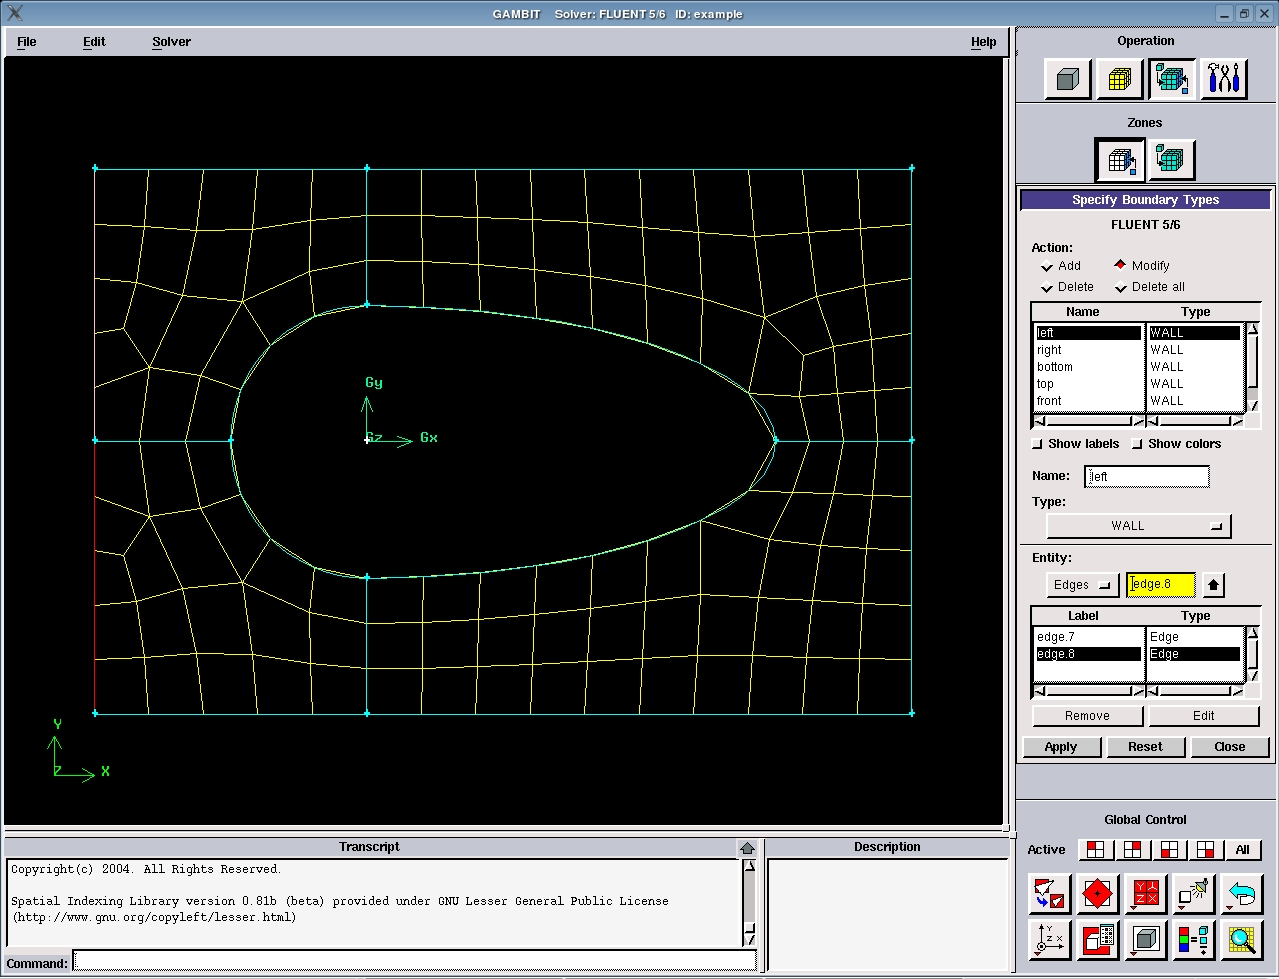
\includegraphics[width=\textwidth]{example01.jpg}
\caption{Defining the boundaries}
\end{figure}

\section{The gambit2semtex input file}

The next step is to create an input file for the converter.
It has to provide the name of grid file and all information 
that is necessary to establish the boundary curves. 
A file matching our example is \verb|example/example.inp|,
which is listed in Figure~\ref{fig:example.inp}.
Looking at this, the experienced reader will recognise that the input data 
is specified in terms of Fortran namelists. 
Lines beginning with \texttt{\#} are comments.

\begin{figure}[th]
\centering
\verbatiminput{example.inp}
\caption{Listing of \texttt{example.inp}.\label{fig:example.inp}}
\end{figure}

The section \texttt{ExportCase} assigns the name of the semtex session
file (\texttt{example}) to the variable \texttt{casename}.
The next section defines the name of the mesh \texttt{file} (\texttt{example.msh}) and the scaling factors \texttt{xScale} and
\texttt{yScale}. These factors can be used to scale the corresponding
point coordinates. If skipped, they are set to $1$ by default. 

The next section defines the boundary curves. 
Here, \texttt{name} refers to the boundary name as specified before in
the gambit session and \texttt{geom} defines the curve type. 
Three choices are possible:
\begin{itemize}
\item \texttt{geom = 1} \quad defines a straight edge,
\item \texttt{geom = 5} \quad a circular arc, and 
\item \texttt{geom = 4} \quad a spline curve.
\end{itemize}
Please notice that other values, e.g. \texttt{geom = 2} or \texttt{geom = 3} 
are invalid!
In case of an arc it is mandatory to provide the
mid point coordinates (\texttt{x0} and \texttt{y0}).

In case of a spline curve (\texttt{geom = 4}) the parameter \texttt{file}
refers to a file containing the $x,y$ coordinates of the spline points
listed line by line. This allows to reuse the vertex file that was
employed in gambit for creating the edge.
However, with the current version it is save to remove the $z$ coordinates 
of the points in this file.
If the specification of \texttt{file} is skipped, the converter generates
a cubic spline from the grid points on this boundary. This spline is used
to create a curve data file for semtex. 
The name of this file is composed of the case name and the boundary name,
e.g. \verb|example_bndry-spline_back.dat| for the boundary named ''back''
in the given example. 
In both cases, a corresponding \verb|CURVE| section is inserted in the
semtex session file.

The final section contains the \verb|Boundary_Condition| entries defining
the semtex boundary groups. Each entry refers to one boundary that is
identified by the \texttt{name} assigned in the gambit session.
The \texttt{key} parameter associates the boundary with one group defined in 
the \texttt{GROUP} section in the session file. It is used to create the
corresponding entries in the \texttt{SURFACES} section. 
Concerning the conventions for choosing the group identifiers we refer to
the semtex userguide. 
Typically  
'\texttt{w}' defines the ''wall group'', while
'\texttt{p}' is reserved to identify periodic boundaries.
In the latter case the parameter \texttt{link} provides the
name of the matching boundary. For instance, in the example given in 
Fig.~\ref{fig:example.inp} the boundaries ''bottom'' and ''top'' refer
to each other.

%Daf"ur gibt es beim Vernetzen der Beiden R"ander in Gambit die Funktion %\verb|Link /| \verb|Unlink edges|, diese ist "uber das Toolpad zu erreichen.

Once the input file is completed, run the converter:

\begin{verbatim}
> gambit2semtex
\end{verbatim}

The program prompts for the name of the input file and creates the
session file in the same directory.

\section{Editing the session file}

To complete the session file, you have to add the sections
\begin{itemize}
\item \texttt{FIELDS}
\item \texttt{TOKENS}
\item \texttt{GROUPS}
\item \texttt{BCS}
\end{itemize}
You should be careful especially with the latter two, because the group
identifiers have to match those referenced in the gambit2semtex
input file. 
For further information we refer to the semtex userguide \cite{semtex}.

\bibliographystyle{unsrt} 
\bibliography{ug}




\end{document}